\documentclass{article}



\usepackage{IEEEtrantools}
\usepackage{amsmath}
\usepackage{mathrsfs}
\usepackage{graphicx}
\usepackage{subcaption}
\usepackage{setspace}
\usepackage{color}
\usepackage[margin=0.7in]{geometry}

\newcommand{\C}{\mathbf{C}}
\newcommand{\h}{\mathbf{h}}
\renewcommand{\r}{\mathbf{r}}
\newcommand{\x}{\mathbf{x}}
\newcommand{\A}{\mathbf{A}}
\newcommand{\Z}{\mathbf{Z}}
\newcommand{\Y}{\mathbf{Y}}
\newcommand{\X}{\mathbf{X}}
\newcommand{\N}{\mathcal{N}}
\newcommand{\w}{\mathbf{w}}
\newcommand{\logit}{\text{logit}}


\begin{document}

  \section{Context}

  \paragraph{Objectives:}

  I want to predict the nutrient flux from the deep sea to the surface layer in the northern Red Sea. This is interesting, because it could give us an idea about the new production. With existing methods, this amount of new production is difficult to estimate without in-situ data. Therefore if there is a method that allows us to do that by just using satellite data, it could be of interest for marine biologist.

  \paragraph{Data:}

  I clustered the red sea into 8 provinces bases on monthly chl data and a Gaussian mixture model clustering algorithm. I am interested in the northernmost cluster during winter 1999-2000 because there is an important bloom in this region. I averaged daily SeaWifs data from December 1999 to May 2000 in the given cluster, giving me the following a time series data.


  \begin{figure}[ht]
  \centering
    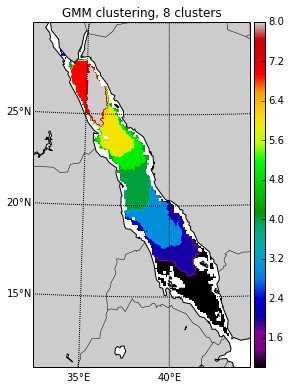
\includegraphics[scale=.3]{./clusters.png}
  \caption{Result of clustering. We are interested in the red region.}
  \end{figure}


  \begin{figure}[ht]
  \centering
    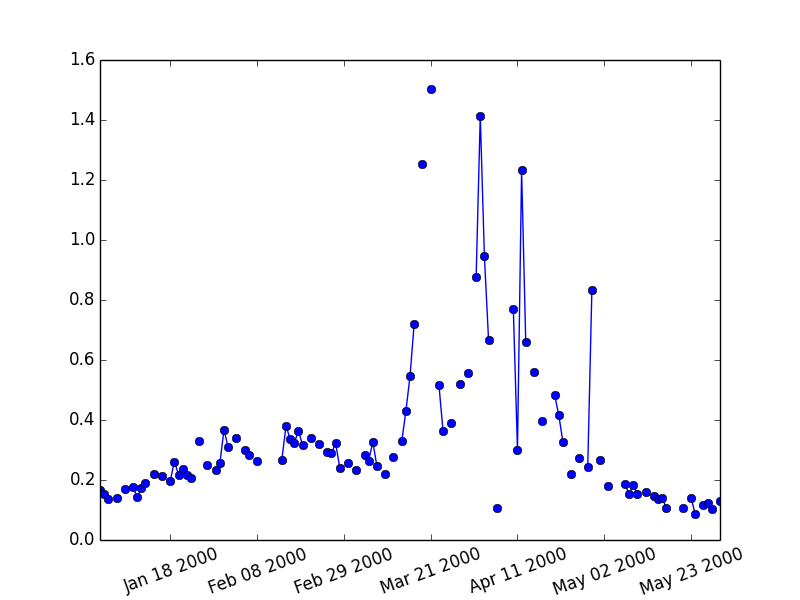
\includegraphics[scale=.3]{./chl_ts.png}
  \caption{Averaged of CHL concentration in studied cluster: The data to be used in the inversion.}
  \end{figure}


  \paragraph{Box model:}

  We assume that a box model or 0d model represents the mixed layer in the cluster region we are interested in, and futhermore that there is no exchange with the neighboring regions and that the input of nutrient just come from the deep sea. We only model the phytoplankton, the nutrient concentration (we assume that the nitrate is the limiting nutrient), and the grazing pressure through a zooplankton concentration. A certain part of the zooplankton and phytoplankton is assumed to be lost by sinking, whereas a stochastic term models a flux of nutrient that diffuse to the mixed layer from the deep water. This is that term that we are interested in estimating.

  \begin{figure}[ht]
  \centering
    \includegraphics[scale=.3]{./model.png}
  \caption{Box model}
  \end{figure}

  \paragraph{NPZ model:}

  The NPZ model is the simplest meaningful model for the phytoplankton
  growth. It is a ODE model that links phytoplankton concentrations 
  (\textcolor{green}{P}) to preying zooplankton (\textcolor{red}{Z}) and
  available nutrient (\textcolor{blue}{N}) concentrations. In our case we 
  augment the NPZ model by including a nutrient flux term ($\Phi$) that 
  models an input of nutrient from the deep sea. The equations of the
  NPZ model are shown below:

  \begin{IEEEeqnarray}{rCl}
    \textcolor{green}{\frac{dP}{dt}} & = & 
    \textcolor{green}{\mu\frac{N}{k+N}P} 
    - \textcolor{red}{gPZ} 
    - \textcolor{green}{\varepsilon_PP}
    - \textcolor{green}{\varepsilon_P^* P^2},\\
    \textcolor{red}{\frac{dZ}{dt}} & = & 
    \textcolor{red}{\gamma gPZ} 
    - \textcolor{red}{\varepsilon_ZZ}
    - \textcolor{red}{\varepsilon_Z^*Z^2},\\
    \textcolor{blue}{\frac{dN}{dt}} & = &
    -\textcolor{green}{\mu\frac{N}{k+N}P} 
    + \textcolor{red}{(1-\gamma)gPZ} 
    + \textcolor{green}{\varepsilon_PP} 
    + \textcolor{red}{\varepsilon_ZZ} 
    + \Phi_N(t).
  \end{IEEEeqnarray}


  \section{State-Space model}

  Denote $Y_1, ..., Y_T$ the observations of chlorophyll
  concentration, $\X_1, ..., \X_T$ the state variables, with
  $\X_t = \left[N_t, P_t, Z_t, \Phi_t\right]^T$, the concentration of each of the
  ODE state variables at time $t$. For now on, we actually considere the log
  of these concentrations. 


  \subparagraph{State Equation:}

  The state variables are assumed Markovian:

  \begin{IEEEeqnarray}{c}
    X_t = \left[
      \begin{array}{c}
        N_t \\P_t\\ Z_t \\ \Phi_t
      \end{array}\right] = 
    \left[\begin{array}{c} f(X_{t-1};\theta)\\ \alpha\Phi_{t-1}
      \end{array}\right] + \w_t, \w_t \sim \N(0, diag(\Gamma))
  \end{IEEEeqnarray}

  $f$ is the result of the integration of the ODE system between times 
  $t-1$ and $t$ with initial conditions $\left[N_{t-1}, P_{t-1}, Z_{t-1}
  \right]$ and a fixed nutrient flux $\Phi_{t-1}$. 
  $\Gamma$ is the noise model covariance. $\theta$ are the NPZ model parameters.
  $\Phi_t$ is an autoregressive process with coeffiction $\alpha = 0.7$.


  \subparagraph{Observation equation:}

  The observations are independent conditionally on the state of the system.

  \begin{IEEEeqnarray}{c}
  	Y_t = c + P_t + w^o_t,
  \end{IEEEeqnarray}

  with $w^o_t \sim \N(0, (\sigma^o)^2)$ iid and $c$ in the log-conversion
  rate between the chlorophyll and the phytoplankton concentrations. 

\section{EM methodology}

$\Theta$ = $\{\Gamma, \sigma_o^2, x_0^b, B\}$ are unknown and estimated by with the iterative Expectation-Maximization algorithm, with latent variable the states $X_{0:T}$. In the E-step, the distribution $p(X_{0:T}|\Theta, Y_{0:T})$ is estimated given the current estimate of the parameters $\Theta$. Since it is a smoothing problem with a non linear model, I use the Ensemble Kalman Smoother. In the M-step, $\Theta$ is updated by maximizing $\log p(\Theta|X_{0:T}, Y_{0:T})$


\section{Problems}

\begin{itemize}
  \item The model needs to be validated by someone who knows about ecological modelling and the biology of the Red Sea. Currently I don't know:
  \begin{itemize}
    \item If a 0d model is appropriate
    \item If the NPZ captures enough of the dynamics
    \item What should be the transfer function and the parameters
    \item If the stochastic nutrient flux assumption is reasonable
  \end{itemize}
  \item With the current model I run frequently into numerical instability issues
  \item The parameter values are unknown, we tried a state-parameter estimation, but it doesn't work except is we start around the true value and put a ridiculous amount of noise. 
\end{itemize}




\end{document}

